\section{Motivating Examples}
\label{sec:examples}

Before explaining SWIN,
we briefly explain the type safety problem in the 
existing systems.
%In this section, 
We shall first briefly describe Twinning \cite{twinning}, 
a typical API adaptation language.
Then, we will
give some examples to show why Twinning cannot preserve the type
correctness in program transformation. Finally, we will informally
present an overview of our work.
%\label{example}
%\begin{figure}
%    \centering
%    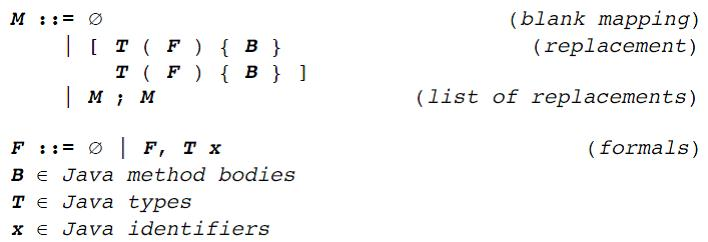
\includegraphics[width=8.5cm]{one}
%    \caption{Syntax of twinning}
%    \label{fig-syntax}
%  \end{figure}

Twinning is a rule-based language for adapting programs between
alternative APIs. The design goal of Twinning is to be easy to use
while allowing a reasonable set of adaptation tasks to be
specified. 
%Figure~\ref{fig-syntax} shows the syntax of Twinning. 
A Twinning program basically consists of a set of replacement rules 
in the form of
\[
\begin{array}{ll}
~[ \\
\tt\quad T_{10} (T_{11}~x_1, \ldots, T_{1n}~x_n)~\{~ \mbox{{\bf return }javaExp}_1;~\}\\
\tt\quad T_{20} (T_{21}~y_1, \ldots, T_{2n}~y_n)~\{~ \mbox{{\bf return }javaExp}_2;~\}\\
~]
\end{array}
\]
which means (1) $T_{1i}$ will be replaced by $T_{2i}$ for all $i$ (the
set of pairs $[T_{1i}, T_{2i}]$ from all replacement rules are called
a \emph{type mapping}); (2) $x_i$ is a meta variable that will match a
Java expression of type $T_{1i}$ in the source code and instantiates
$y_i$ with that expression;
(3)
$\mbox{javaExp}_1$, which is a Java expression of type $T_{10}$ that uses meta 
variables $x_1\ldots x_n$, will be used to match Java expressions, and these
expressions will be replaced by $\mbox{javaExp}_2$ of type $T_{20}$, where the meta
variables $y_i$ are instantiated with the matched expressions by $x_1\ldots x_n$
% Java expressions matched by
% $\mbox{javaExp}_1$ that uses meta variables $x_i$ and has type
% $T_{10}$ will be replaced by Java expression
% $\mbox{javaExp}_2$ that uses meta variables $y_i$ and has type
% $T_{20}$
\footnote{Strictly speaking, Twinning also allows replacing a
  block of statements rather than a single expression. For the ease of
  presentation, we shall only consider expression replacement in this
  paper. All discussions apply to statements replacement as well.}.
%
%
%\begin{example}[Replacement Rule]
%  \rm

As a simple example, consider the following replacement rule
\begin{quote}
\begin{lstlisting}[numbers=left]
[ 
 Enumeration(Hashtable x) 
  {return x.elements();}
 Iterator(HashMap x) 
  {return x.values().iterator();} 
]
\end{lstlisting}
\end{quote}
which will match any call to \code{elements} in class \code{Hashtable}, and replace it by a call to \code{values().iterator()} in class \code{HashMap}. 
%The expression after the
%first \code{return} in line 3 will be used to match an expression in
%the Java code, where the variable \code{x} is a meta variable used to
%match a Java variable of type \code{Hashtable}. The expression after
%the \code{return} in line 5 will be used to replace any matched
%expression, where the meta variable \code{x} will be replaced by the
%name of the matched Java variable. The return type \code{Enumeration} in line
%2 and the return type \code{Iterator} in line 4 are used to declare the
%return types of the expressions to ease the type analysis of the
%language.
For instance, given the following piece of code,
\begin{quote}
\begin{lstlisting}
void f(Hashtable t) {
  Enumeration e = t.elements():
  ...
}
\end{lstlisting}
\end{quote}
the replacement rule will produce the following piece of code, where
the meta variable \code{x} in the replacement rule matches the expression \code{t}.
\begin{quote}
\begin{lstlisting}
void f(HashMap t) {
  Iterator e = t.values().iterator():
  ...
}
\end{lstlisting}
\end{quote}
%\myendup
%\end{example}

%Besides replacing method calls, Twinning also collect a type mapping
%from all replacements, and the type mapping is collected from the
%return types of the replacement and the types of the pointwisely
%corresponding meta variables. The above example declares two pairs for
%the type mapping. One is from the return type, mapping \code{Enumeration} to
%\code{Iterator}, and the other one is from the declaration of the meta
%variable $x$, mapping \code{Hashtable} to \code{HashMap}. After
%collecting the type mapping, Twinning will replace the type uses in
%the Java source code according to the type mapping. In this case, all
%type occurrences of \code{Enumeration} in the Java code will be
%replaced as \code{Iterator}, and all type occurrences \code{Hashtable}
%will be replaced as \code{HashMap}. 


Twinning mainly checks two conditions to avoid introducing new type errors
in the code. First, Twinning requires each replacement must be
well typed under the typing rules of Java. In this way, we can
ensure the replacement of expressions does not introduce new type 
errors. Second, Twinning requires that one type is only mapped to
one type in the type mapping (i.e., one type cannot be mapped to different types by 
replacement rules). This condition ensures that the replacement of
types can be correctly performed.

Unfortunately, these two conditions cannot fully ensure type safety. 
First, \yxmodifyok{Twinning cannot guarantee subtyping preservation.}{type errors may be
introduced when subtyping relations are
involved.} 
%
% Though the checking rules of Twinning are quite reasonable, these
%rules alone cannot ensure type safety. 
To see this, consider a
practical example to adapt
programs from Java Swing API to SWT API~\cite{icsm2010}, where 
 the correspondences between types of
the two APIs are summarized in Figure~\ref{fig-swingtoswt},
and the following presents part of the rules for replacing 
type constructors to their counterparts.
\begin{quote}
\begin{lstlisting}
[ 
 Container () {return new Container();}
 Composite () 
  {return new Composite(new Shell(), 0);}
]

[ JList () { return new JList(); } 
  List  () { return new List(); } ]
\end{lstlisting}
\end{quote}
%
%[ JFrame () { return new JFrame(); }
%  Shell () { return new Shell(); } ]
%These rules replaces  Some constructors on the SWT side have more parameters
%than those in Swing, so we provide default values for these constructors.
% \noindent PAR and N are default values provided for constructor of class Composite.
% It seems right while using these rules to update clients with API Swing, 
% but consider following statement in a type-safety client program:
The typing problem happens if we apply the above rules to the following piece of code:
\begin{quote}
\begin{lstlisting}[language=Java]
Container x = new JList();
\end{lstlisting}
\end{quote}
Clearly, it will yield the code
%
%If we transform this statement with rules above, it will replace the
%constructor call to \code{JList()} with a call to \code{List()}, and
%replace \code{Container} with \code{Composite}. The transformed client
%code is shown as follows.
\begin{quote}
\begin{lstlisting}[language=Java]
Composite x = new List(); 
\end{lstlisting}
\end{quote}
which actually contains a type error:
JList is a subtype of Container, but List is not a subtype of
Composite, so we cannot assign a \code{List} object to a
\code{Composite} variable. This example shows that, although the two
conditions used in Twinning ensure the replacement of expressions and the
replacement of types are correct by themselves, the {\em intersection} of
the two replacements would introduce type errors.

\begin{figure}
    \centering
    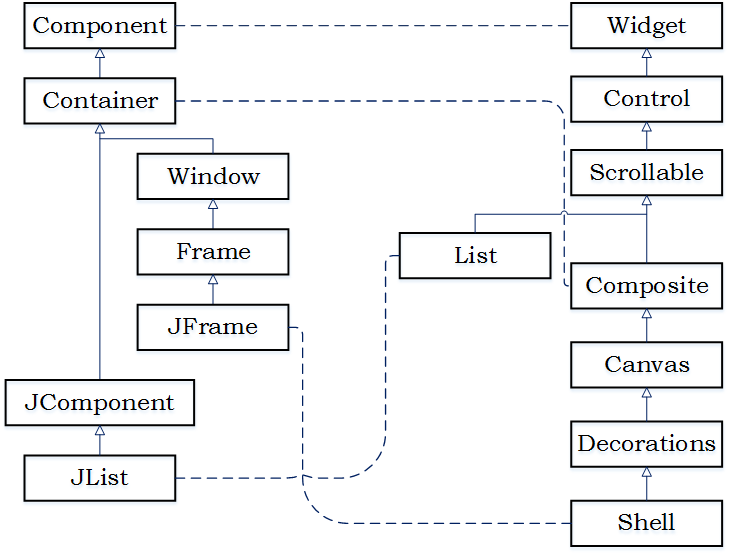
\includegraphics[width=7cm]{swingtoswt}
    \caption{Swing and SWT Type Mapping} 
    \label{fig-swingtoswt}
\end{figure}

% . The cast of type List
% to type Composite is a wrong cast, so the rules above cannot preserve the type correctness.
% In our work, these rules will be excluded.

%The above example shows that the constraints of twinning is not enough to preserve the type
%correctness while updating programs. 

Second, Twinning has no guarantee
% that all components appeared only in the old API are
% fully replaced by components in the new API.
the replacement rules cover all necessary changes.
When there are components appearing only in the old API but are not
transformed by any transformation rule, type errors may be introduced.
% This would introduce type errors when an old component exists in an updated program.
For instance, consider the upgrade of Java SDK from v1.0
to v1.2: class \code{Hashtable} (Figure~\ref{fig:hashtable}) is replaced by
\code{HashMap} (Figure~\ref{fig:hashmap}). For this change, we write a set of 
replacement rules (Figure~\ref{fig:table2map}).
%
%From these rules, we can see method \textit{elements} in class Hashtable
%maps to two methods \textit{values} in class HashMap and \textit{iterator} in
%class Collection. We also require the bodies of these rules can be type checked,
%and the type mapping is a function as twinning. 
To be sure that any program using \code{Hashtable} can be transformed 
in a type-safe way, we must guarantee that all methods and classes in
\code{Hashtable} have their replacements. However, the method \code{contains}
in class \code{Hashtable} has no such replacements in the 
above set of rules. % This means that type-safety requires taking
% account of the difference between the old API and the new API.
%\todo{We can separate the following as the third problem. One reviewer
  %complained that he could not understand our solution to this problem,
  %but I think this is because he missed the problem.} Another more subtle case is that when one replacement declares a type
%change but there is no rule to implement that change. For example, let
%us remove the first rule in Figure~\ref{fig:table2map}. The
%application of the second rule will always introduce a type error
%because the expression matched by \code{x} will never be transformed
%and remains to have type \code{Hashtable}.

\begin{figure}
\begin{lstlisting}[language=java]
class Hashtable {
    Enumeration elements() { }
    boolean contains(Object v) { }
    ...
}
class Enumeration {
    ...
}
\end{lstlisting}
\caption{Hashtable API}
\label{fig:hashtable}
\end{figure}
    % boolean hasMoreElements() { }
    % Object nextElement() { }

\begin{figure}
\begin{lstlisting}[language=java]
class HashMap {
    Collection values() { }            
    boolean containsValue(Object v) { }
    ...
}
class Collection {
    Iterator iterator() { }
    ...
}
class Iterator {
    ...
}
\end{lstlisting}
\caption{HashMap API}
\label{fig:hashmap}
\end{figure}
    % boolean hasNext() { }
    % Object next() { }


\begin{figure}
\begin{lstlisting}
[ Hashtable () { return new Hashtable();}
  HashMap () { return new HashMap(); } ]

[ Enumeration (Hashtable x) 
    { return x.elements(); }
  Iterator (HashMap x) 
    { return x.values().iterator(); } ]
\end{lstlisting}
\caption{Replacement Rules From Hashtable to HashMap}
\label{fig:table2map}
\end{figure}

% [ boolean (Enumeration v) 
%     { return v.hasMoreElements(); }
%   boolean (Iterator v) 
%     { return v.hasNext(); } ]

% [ Object (Enumeration v) 
%     { return v.nextElement(); }
%   Object (Iterator v) 
%     { return v.next(); } ]

In summary, the conditions of Twinning are not
enough to ensure type-safety of the transformation program. We need
the additional conditions to prevent the above two cases. For the first
case, we need to ensure that  the type mapping does not break the
subtyping relations. For the second case, we need to ensure the
replacements cover the full API changes. Putting them together with
the original two conditions from Twinning, we
have the following four conditions.
\begin{itemize}
\item For each code snippet introduced in a replacement rule, the code
  snippet itself must be well typed.
\item The type mapping must form a function, i.e., no type in the
  source API is mapped to two or more types in the target API.
\item The type mapping must preserve the subtyping relation. If $X$ is
  a subtype of $Y$ in the source API and $m$ is the mapping, $m(X)$
  must be a subtype of $m(Y)$ in the target API.
\item % For any method $m$ or field $f$ in the source API, if $m$ or $f$ does
  % not exist in the target API, there must exist a replacement rule
  % matching $m$ or $f$.
  The replacement rules must cover all type changes between the source
  API and target API, 
  %\todo{we should also separate the rest part as a
    %new rule, and change all text in the paper accordingly.(4 rules $\rightarrow$
  %5 rules)} 
  as well as any type changes declared in the type mapping.
\end{itemize}

It will be interesting to see later that these four conditions are
sufficient to ensure type safety. However, as Twinning is presented
informally in the original publication \cite{twinning}, to reason about
type safety,
we need to first build a formal model of the Twinning semantics. A
particular challenge of presenting this formal model is to understand
how the replacement rules can be sequentially applied. For example, to
transform the following piece of code
\begin{quote}
\begin{lstlisting}
new Hashtable().elements()
\end{lstlisting}
\end{quote}
into
\begin{quote}
\begin{lstlisting}
new HashMap().values().iterator()
\end{lstlisting}
\end{quote}
we need to begin with the second rule in
Figure~\ref{fig:table2map} to replace ``\code{elements()}'' and then apply
the first rule to replace ``\code{new Hashtable()}''. If we begin with the
first rule, we shall get an expression
\begin{quote}
\begin{lstlisting}
new HashMap().elements()
\end{lstlisting}
\end{quote}
where the second rule cannot be applied because ``\code{new
  HashMap()}'' has a type \code{HashMap} that cannot be matched by the meta
variable \code{x} of type \code{Hashtable}. In other words, the
transformation is not \emph{confluent} since applying the rules in
different orders gives us different results.

A related issue is that some sequences of rule applications may be
infinite. For example, let us consider the following rule.
\begin{quote}
\begin{lstlisting}
[A (A x) {return x.a();} 
 A (A x) {return x.a().a();]
\end{lstlisting}
\end{quote}
Since the target side of the right also contains the call to
\code{a()}, the rule can be applied again after the transformation,
forming a \emph{non-terminating} transformation.
A terminating and confluent transformation is called a {\em
  convergent} transformation.
A well-formed transformation language should always produce 
convergent transformations. 
However, the publication on Twinning
\cite{twinning} provides no information how Twinning deals with these
issues.

Another usability issue of Twinning is that Twinning allows only exact
type matching, i.e., a meta variable of type $T$ matches a Java
expression only when the expression has exactly type $T$ but not a subtype of $T$. This design eases the
analysis as we can infer all type changes from the type mapping, but
also makes transformation more difficult to write. For example, in
Java v1.0 class \code{Properties} is a sub class of \code{Hashtable},
and thus any call to \code{Properties.elements()} should be
transformed in the same way as \code{Hashtable.elements()}. However,
the second rule in Figure~\ref{fig:table2map} does not apply to calls
to \code{Properties.elements()} because the meta variable \code{x}
has type \code{Hashtable}. As a result, for any replacement rule for a
class $\tt C$, we need to repeat the rule for each sub class of $\tt C$, which
is quite tedious.

To overcome this problem, we design a new language, SWIN (Safe
tWINning). SWIN is based on Twinning but with the following
differences.
\begin{itemize}
\item SWIN has full formal semantics.
  \item SWIN has more flexible rule
application behavior, allowing a meta
variable to match an expression of its sub type.

\item SWIN is convergent. A well typed SWIN program can act on any 
    Java program confluently and free from non-terminating problems.
%\item SWIN employs a normal order evaluation semantics. First, the evaluation rules visit
    %a term leftmost and outermost. After performing the transformation on that term, the evaluation 
    %rules recursively visit the sub terms of the term, and for each visit, the transformation
    %will be applied on the original sub terms, and produce the transformation result by combining
    %the transformed sub terms. This strategy guarantees that the evaluation process is free from
    %confluence and termination problems, as each program element is transformed at most once.
%\item SWIN employs a ``match all, transform once'' semantics. The
  %source program is first matched by the rules and then the
  %replacements of all matches are performed simultaneously. In this way we
  %have no sequential application of rules, effectively avoiding the
  %confluence and termination problem.
%   employs
% a strict top-down order of rule applications, ensuring the
% transformation to be confluent and terminating.
\item SWIN
includes a set of type checking rules checking the four conditions presented
above.
\end{itemize}
In the following sections we shall introduce SWIN formally and
present our proof of type safety.

%These rules will serve as the basis 
%of our new type-safe Java program adaptation framework.

% . In the next section we shall formally show that they are. 


%  Now the question is whether the four rules are enough to ensure type
%  safety. In the next section we shall formally show that they are. 

% From these examples, we can see that invalid or incomplete rules in twinning 
% may introduce type-errors
% while updating client programs. In our paper, we should exclude invalid rules, 
% and assure the all the valid rules in SWIN can preserve the type
% correctness while updating any type-safety programs. 
% In our paper, we give a set of properties that a type safe rule
% should satisfy with, and we call these properties are type safe properties 
% (short for safe properties). There are mainly three properties that rules
% should satisfy with. Next, we will informally and briefly explain these two cases. 

% Consider a rule:
% \begin{align*}
%     [ \quad &T_{1} \quad ( \bar{F} \quad \bar{x} ) \quad \{ \quad B_{1} \quad \} \\
%      &T_{2} \quad ( \bar{G} \quad \bar{y}) \quad \{ \quad B_{2} \quad \} \quad]
%  \end{align*}
%  In rules above, $\bar{F}\; \bar{x}$ is short for $F_{1}\;x_{1},F_{2}\;x_{2},\cdots,F_{n}\;x_{n}$,
%  same as $\bar{G}\;\bar{y}$. 

%  \begin{itemize}
%      \item In rule checking, first, it require that all the variables in
%  $B_{1}$ should be binded with $\bar{x}$, and all the $\bar{x}$ are apperance in $B_{1}$. Second, it 
%  need to assure that $B_{1}$ is a single body, 
%  it means there is no more than one method invoke in $B_{1}$.

%     \item We also collect the type mapping as twinning, and these type mapping should be a 
%         funtion. All the methods in rules should cover all the methods in class appeared in rules, and
%         for the methods in rules should type-safety according the definition of APIs. For any method
%         not in rules, there should be a method in mapped class with same name, and the type of
%         parameters and return value should satisfy the type mapping.

%     \item The last properties is about inheritance. For the inheritance of classes in former API, 
%         these relationship cannot be removed in new API of between any two classes after updated, and
%         the adding of relationship between classes is allowed.
% \end{itemize}


%%% Local Variables: 
%%% mode: latex
%%% TeX-master: "pepm-15"
%%% End: 
